\section{SPARQL queries and symbolic reasoning}\label{sec:sparql}

\subsection{Rules R1--R7 as SPARQL Update}
Points, NRR and qualification need arithmetic and counting, which OWL cannot express, so they are implemented
as SPARQL~1.1 Update rules \citep{w3c2013sparqlupdate} that materialise one \texttt{qp:StandingEntry} per team.
They run after OWL~2~RL reasoning, because they rely on inferred facts such as \texttt{CompletedMatch} and
\texttt{participatesIn}.

\begin{table}[H]\centering\small
\begin{tabular}{p{1.3cm}p{13.6cm}}
\toprule
\textbf{Rule} & \textbf{Definition} \\ \midrule
R1 & points $=$ won $\times$ pointsForWin $+$ lost $\times$ pointsForLoss $+$ noResult $\times$ pointsForNoResult \\
R2 & NRR $=$ runs scored / overs faced $-$ runs conceded / overs bowled (overs $=$ balls/6; all out $=$ full quota; shortened matches use \texttt{oversPerSide}) \\
R3 & maxReachablePoints $=$ points $+$ remaining fixtures $\times$ pointsForWin \\
R4 & EliminatedStanding if at least \emph{qualifyingPlaces} other teams already have more points than this team can reach \\
R5 & QualifiedStanding if fewer than \emph{qualifyingPlaces} other teams can still reach this team's points \\
R6 & InContentionStanding otherwise \\
R7 & position: more points, then more wins (tie-break 1), then higher NRR (tie-break 2) \\
\bottomrule
\end{tabular}
\caption{SPARQL Update rules (\texttt{SPARQL\_Queries/rules/}). R4 and R5 use points only, so they never
wrongly declare a team qualified or eliminated, but may keep a team ``in contention'' longer than the official
table.}
\end{table}

\lstinputlisting[language=SPARQL,caption={Rule R7 (position with the IPL tie-break order).}]{generated/queries/R7_position.ru}

The derived league table (\tabref{tab:standings}) is identical to the official IPL table after match~39.

\begin{table}[H]\centering
{\small
\begin{tabular}{rlrrl}
\toprule
\textbf{position} & \textbf{team} & \textbf{points} & \textbf{netRunRate} & \textbf{inQualifyingPlace} \\
\midrule
1 & PBKS & 13 & 1.333 & True \\
2 & RCB & 12 & 1.919 & True \\
3 & SRH & 10 & 0.815 & True \\
4 & RR & 10 & 0.602 & True \\
5 & GT & 8 & -0.475 & False \\
6 & CSK & 6 & -0.121 & False \\
7 & DC & 6 & -1.06 & False \\
8 & KKR & 5 & -0.751 & False \\
9 & MI & 4 & -0.736 & False \\
10 & LSG & 4 & -1.106 & False \\
\bottomrule
\end{tabular}}

\caption{League positions derived by rules R1--R7 (query Q04).}\label{tab:standings}
\end{table}

\subsection{The eleven SPARQL queries}
\begin{table}[H]\centering\small
\begin{tabular}{p{4.2cm}p{10.6cm}}
\toprule
\textbf{Required feature} & \textbf{Queries} \\ \midrule
Basic graph pattern & Q01 \\
FILTER & Q05, Q06, Q09, Q11 \\
OPTIONAL / UNION & Q03 (OPTIONAL), Q09 (UNION and OPTIONAL) \\
Aggregation & Q02, Q03, Q10 (with HAVING) \\
Multi-hop traversal & Q05, Q07, Q11 \\
Property paths & Q01, Q04, Q05, Q07 (inverse path \texttt{\^{}qp:hasWinner}) \\
Inference-dependent & Q02, Q08 (and rule-derived classes in Q04, Q06, Q11) \\
\bottomrule
\end{tabular}
\caption{SPARQL feature coverage.}
\end{table}

Every query below was run on the graph after OWL~2~RL reasoning and the rules; the same results are returned by
GraphDB (\figref{fig:graphdb_sparql_Q05.jpg}, \figref{fig:graphdb_sparql_Q04.jpg}).

\subsubsection*{Q01 --- season rules (CQ15; basic graph pattern, property path)}
\lstinputlisting[language=SPARQL]{generated/queries/Q01_season_rules.rq}
\noindent\textit{Output (2 rows):}\par\smallskip
\resizebox{\ifdim\width>\linewidth\linewidth\else\width\fi}{!}{{\footnotesize
\begin{tabular}{llllllll}
\toprule
\textbf{season} & \textbf{pointsForWin} & \textbf{pointsForLoss} & \textbf{pointsForNoResult} & \textbf{oversQuota} & \textbf{qualifyingPlaces} & \textbf{tieBreakRank} & \textbf{tieBreak} \\
\midrule
IPL 2026 & 2 & 0 & 1 & 20 & 4 & 1 & Most wins \\
IPL 2026 & 2 & 0 & 1 & 20 & 4 & 2 & Net run rate \\
\bottomrule
\end{tabular}}}
\medskip
\subsubsection*{Q02 --- points table (CQ1; aggregation, inference-dependent)}
\lstinputlisting[language=SPARQL]{generated/queries/Q02_points_table.rq}
\noindent\textit{Output (10 rows):}\par\smallskip
\resizebox{\ifdim\width>\linewidth\linewidth\else\width\fi}{!}{{\footnotesize
\begin{tabular}{llllll}
\toprule
\textbf{team} & \textbf{played} & \textbf{won} & \textbf{lost} & \textbf{noResult} & \textbf{points} \\
\midrule
PBKS & 7 & 6 & 0 & 1 & 13 \\
RCB & 8 & 6 & 2 & 0 & 12 \\
RR & 8 & 5 & 3 & 0 & 10 \\
SRH & 8 & 5 & 3 & 0 & 10 \\
GT & 8 & 4 & 4 & 0 & 8 \\
CSK & 8 & 3 & 5 & 0 & 6 \\
DC & 8 & 3 & 5 & 0 & 6 \\
KKR & 8 & 2 & 5 & 1 & 5 \\
\multicolumn{6}{l}{\textit{\ldots{} 2 more rows}} \\
\bottomrule
\end{tabular}}}
\medskip
\subsubsection*{Q03 --- net run rate (CQ3; aggregation, OPTIONAL, VALUES)}
\lstinputlisting[language=SPARQL]{generated/queries/Q03_net_run_rate.rq}
\noindent\textit{Output (10 rows):}\par\smallskip
\resizebox{\ifdim\width>\linewidth\linewidth\else\width\fi}{!}{{\footnotesize
\begin{tabular}{llllll}
\toprule
\textbf{team} & \textbf{runsFor} & \textbf{ballsFaced} & \textbf{runsAgainst} & \textbf{ballsBowled} & \textbf{netRunRate} \\
\midrule
RCB & 1501 & 817 & 1437 & 947 & 1.919 \\
PBKS & 1315 & 672 & 1249 & 720 & 1.333 \\
SRH & 1683 & 951 & 1513 & 926 & 0.815 \\
RR & 1391 & 847 & 1380 & 895 & 0.602 \\
CSK & 1496 & 960 & 1397 & 885 & -0.121 \\
GT & 1389 & 930 & 1491 & 948 & -0.475 \\
MI & 1229 & 781 & 1279 & 754 & -0.736 \\
KKR & 1218 & 838 & 1315 & 833 & -0.751 \\
\multicolumn{6}{l}{\textit{\ldots{} 2 more rows}} \\
\bottomrule
\end{tabular}}}
\medskip
\subsubsection*{Q04 --- qualifying places (CQ2; property path, rule results)}
\lstinputlisting[language=SPARQL]{generated/queries/Q04_qualifying_places.rq}
\noindent\textit{Output (10 rows):}\par\smallskip
\resizebox{\ifdim\width>\linewidth\linewidth\else\width\fi}{!}{{\footnotesize
\begin{tabular}{lllll}
\toprule
\textbf{position} & \textbf{team} & \textbf{points} & \textbf{netRunRate} & \textbf{inQualifyingPlace} \\
\midrule
1 & PBKS & 13 & 1.333 & True \\
2 & RCB & 12 & 1.919 & True \\
3 & SRH & 10 & 0.815 & True \\
4 & RR & 10 & 0.602 & True \\
5 & GT & 8 & -0.475 & False \\
6 & CSK & 6 & -0.121 & False \\
7 & DC & 6 & -1.06 & False \\
8 & KKR & 5 & -0.751 & False \\
\multicolumn{5}{l}{\textit{\ldots{} 2 more rows}} \\
\bottomrule
\end{tabular}}}
\medskip
\subsubsection*{Q05 --- remaining fixtures (CQ4; multi-hop, FILTER, property path)}
\lstinputlisting[language=SPARQL]{generated/queries/Q05_remaining_fixtures.rq}
\noindent\textit{Output (6 rows):}\par\smallskip
\resizebox{\ifdim\width>\linewidth\linewidth\else\width\fi}{!}{{\footnotesize
\begin{tabular}{lllll}
\toprule
\textbf{matchNumber} & \textbf{date} & \textbf{opponent} & \textbf{venue} & \textbf{city} \\
\midrule
40 & 2026-04-28 & PBKS & Maharaja Yadavindra Singh International Cricket Stadium & Mullanpur \\
43 & 2026-05-01 & DC & Sawai Mansingh Stadium & Jaipur \\
52 & 2026-05-09 & GT & Sawai Mansingh Stadium & Jaipur \\
62 & 2026-05-17 & DC & Arun Jaitley Stadium & New Delhi \\
64 & 2026-05-19 & LSG & Sawai Mansingh Stadium & Jaipur \\
69 & 2026-05-24 & MI & Wankhede Stadium & Mumbai \\
\bottomrule
\end{tabular}}}
\medskip
\subsubsection*{Q06 --- qualification status (CQ5--CQ7; rule-inferred classes, FILTER)}
\lstinputlisting[language=SPARQL]{generated/queries/Q06_qualification_status.rq}
\noindent\textit{Output (10 rows):}\par\smallskip
\resizebox{\ifdim\width>\linewidth\linewidth\else\width\fi}{!}{{\footnotesize
\begin{tabular}{lllll}
\toprule
\textbf{team} & \textbf{points} & \textbf{remainingFixtures} & \textbf{maxReachablePoints} & \textbf{status} \\
\midrule
PBKS & 13 & 7 & 27 & In-contention standing \\
RCB & 12 & 6 & 24 & In-contention standing \\
SRH & 10 & 6 & 22 & In-contention standing \\
RR & 10 & 6 & 22 & In-contention standing \\
GT & 8 & 6 & 20 & In-contention standing \\
CSK & 6 & 6 & 18 & In-contention standing \\
DC & 6 & 6 & 18 & In-contention standing \\
KKR & 5 & 6 & 17 & In-contention standing \\
\multicolumn{5}{l}{\textit{\ldots{} 2 more rows}} \\
\bottomrule
\end{tabular}}}
\medskip
\subsubsection*{Q07 --- teams beaten (CQ11; multi-hop, inverse property path)}
\lstinputlisting[language=SPARQL]{generated/queries/Q07_teams_beaten.rq}
\noindent\textit{Output (5 rows):}\par\smallskip
\resizebox{\ifdim\width>\linewidth\linewidth\else\width\fi}{!}{{\footnotesize
\begin{tabular}{lllll}
\toprule
\textbf{matchNumber} & \textbf{date} & \textbf{beaten} & \textbf{venue} & \textbf{city} \\
\midrule
3 & 2026-03-30 & CSK & Barsapara Cricket Stadium & Guwahati \\
9 & 2026-04-04 & GT & Narendra Modi Stadium & Ahmedabad \\
13 & 2026-04-07 & MI & Barsapara Cricket Stadium & Guwahati \\
16 & 2026-04-10 & RCB & Barsapara Cricket Stadium & Guwahati \\
32 & 2026-04-22 & LSG & Bharat Ratna Shri Atal Bihari Vajpayee Ekana Cricket Stadium & Lucknow \\
\bottomrule
\end{tabular}}}
\medskip
\subsubsection*{Q08 --- venues played (CQ13; inference-dependent (property chain))}
\lstinputlisting[language=SPARQL]{generated/queries/Q08_venues_played.rq}
\noindent\textit{Output (6 rows):}\par\smallskip
\resizebox{\ifdim\width>\linewidth\linewidth\else\width\fi}{!}{{\footnotesize
\begin{tabular}{ll}
\toprule
\textbf{venue} & \textbf{city} \\
\midrule
Narendra Modi Stadium & Ahmedabad \\
Barsapara Cricket Stadium & Guwahati \\
Rajiv Gandhi International Stadium & Hyderabad \\
Sawai Mansingh Stadium & Jaipur \\
Eden Gardens & Kolkata \\
Bharat Ratna Shri Atal Bihari Vajpayee Ekana Cricket Stadium & Lucknow \\
\bottomrule
\end{tabular}}}
\medskip
\subsubsection*{Q09 --- team results (CQ12; UNION, OPTIONAL, FILTER)}
\lstinputlisting[language=SPARQL]{generated/queries/Q09_team_results.rq}
\noindent\textit{Output (8 rows):}\par\smallskip
\resizebox{\ifdim\width>\linewidth\linewidth\else\width\fi}{!}{{\footnotesize
\begin{tabular}{llllll}
\toprule
\textbf{matchNumber} & \textbf{date} & \textbf{opponent} & \textbf{result} & \textbf{points} & \textbf{shortenedTo} \\
\midrule
2 & 2026-03-29 & MI & Lost & 0 &  \\
6 & 2026-04-02 & SRH & Lost & 0 &  \\
12 & 2026-04-06 & PBKS & No result & 1 &  \\
15 & 2026-04-09 & LSG & Lost & 0 &  \\
22 & 2026-04-14 & CSK & Lost & 0 &  \\
25 & 2026-04-17 & GT & Lost & 0 &  \\
28 & 2026-04-19 & RR & Won & 2 &  \\
38 & 2026-04-26 & LSG & Won & 2 &  \\
\bottomrule
\end{tabular}}}
\medskip
\subsubsection*{Q10 --- home win ratio (CQ14; aggregation with HAVING)}
\lstinputlisting[language=SPARQL]{generated/queries/Q10_home_win_ratio.rq}
\noindent\textit{Output (6 rows):}\par\smallskip
\resizebox{\ifdim\width>\linewidth\linewidth\else\width\fi}{!}{{\footnotesize
\begin{tabular}{llll}
\toprule
\textbf{team} & \textbf{homeMatches} & \textbf{homeWins} & \textbf{winPercent} \\
\midrule
PBKS & 3 & 3 & 100 \\
RCB & 5 & 4 & 80 \\
RR & 4 & 3 & 75 \\
SRH & 4 & 3 & 75 \\
CSK & 3 & 2 & 67 \\
GT & 4 & 2 & 50 \\
\bottomrule
\end{tabular}}}
\medskip
\subsubsection*{Q11 --- rival fixtures (CQ8--CQ9; multi-hop, rule-inferred class)}
\lstinputlisting[language=SPARQL]{generated/queries/Q11_rival_fixtures.rq}
\noindent\textit{Output (6 rows):}\par\smallskip
\resizebox{\ifdim\width>\linewidth\linewidth\else\width\fi}{!}{{\footnotesize
\begin{tabular}{lllllll}
\toprule
\textbf{matchNumber} & \textbf{date} & \textbf{opponent} & \textbf{opponentPosition} & \textbf{opponentPoints} & \textbf{rrPoints} & \textbf{pointsGap} \\
\midrule
52 & 2026-05-09 & GT & 5 & 8 & 10 & 2 \\
40 & 2026-04-28 & PBKS & 1 & 13 & 10 & 3 \\
43 & 2026-05-01 & DC & 7 & 6 & 10 & 4 \\
62 & 2026-05-17 & DC & 7 & 6 & 10 & 4 \\
64 & 2026-05-19 & LSG & 10 & 4 & 10 & 6 \\
69 & 2026-05-24 & MI & 9 & 4 & 10 & 6 \\
\bottomrule
\end{tabular}}}
\medskip


\shot[0.95\linewidth]{graphdb_sparql_Q05.jpg}{Multi-hop query Q05 executed in GraphDB: RR's six remaining
fixtures with opponents, dates, venues and cities.}
\shot[0.95\linewidth]{graphdb_sparql_Q04.jpg}{Q04 in GraphDB: positions 1--10 match the official table.}

\subsection{Symbolic inference examples}
Each example follows the pattern \emph{explicit facts $\rightarrow$ rule or schema knowledge $\rightarrow$
inferred fact}, and is demonstrated by running the same query with inference switched off and on.

\paragraph{Example 1 --- the winner of a match took part in it (O1).}
Explicit: \texttt{match:IPL-2026-M01 qp:hasWinner team:RCB ; qp:hasLoser team:SRH}.
Rule: \texttt{hasWinner} and \texttt{hasLoser} are sub-properties of \texttt{hasParticipant}.
Inferred: \texttt{match:IPL-2026-M01 qp:hasParticipant team:RCB, team:SRH}. All 76 participation links of
decided matches are inferred this way.

\paragraph{Example 2 --- a match with a winner is a completed match (O3, O4).}
Explicit: \texttt{match:IPL-2026-M01 a qp:Match ; qp:hasWinner team:RCB}.
Rules: the domain of \texttt{hasWinner} is \texttt{DecidedMatch}, and \texttt{DecidedMatch} is a subclass of
\texttt{CompletedMatch}. Inferred: match~1 is a \texttt{DecidedMatch} and a \texttt{CompletedMatch}.
Season-wide, 0 completed matches are stored and 39 are inferred; the points table (Q02) depends on this.

\paragraph{Example 3 --- the venues a team has played at (O1, O2, O5).}
Explicit: \texttt{match:IPL-2026-M03 qp:hasWinner team:RR ; qp:playedAt venue:barsapara-cricket-stadium}.
Rules: sub-property (O1), inverse (O2) and the chain \texttt{playedAtVenue $\equiv$ participatesIn $\circ$ playedAt} (O5).
Inferred: \texttt{team:RR qp:participatesIn match:IPL-2026-M03} and
\texttt{team:RR qp:playedAtVenue venue:barsapara-cricket-stadium}. Season-wide, 0 team--venue links are stored
and 50 are inferred.

\begin{table}[H]\centering
{\footnotesize
\begin{tabular}{lrrp{8.2cm}}
\toprule
\textbf{Query} & \textbf{Off} & \textbf{On} & \textbf{Values with inference} \\
\midrule
I1\_winner\_is\_participant & 0 & 2 & RCB; SRH \\
I2\_match\_classified\_completed & 1 & 3 & qp:CompletedMatch; qp:DecidedMatch; qp:Match \\
I3\_team\_played\_at\_venue & 0 & 6 & Barsapara Cricket Stadium; Bharat Ratna Shri Atal Bihari Vajpayee Ekana Cricket Stadium; E... \\
season-wide (explicit) &  &  & CompletedMatch=0, DecidedMatch=0, team-venue pairs=0 \\
season-wide (inferred) &  &  & CompletedMatch=39, DecidedMatch=38, team-venue pairs=50 \\
\bottomrule
\end{tabular}}

\caption{Inference demonstrations I1--I3: rows returned with inference off and on.}
\end{table}

\begin{figure}[H]\centering
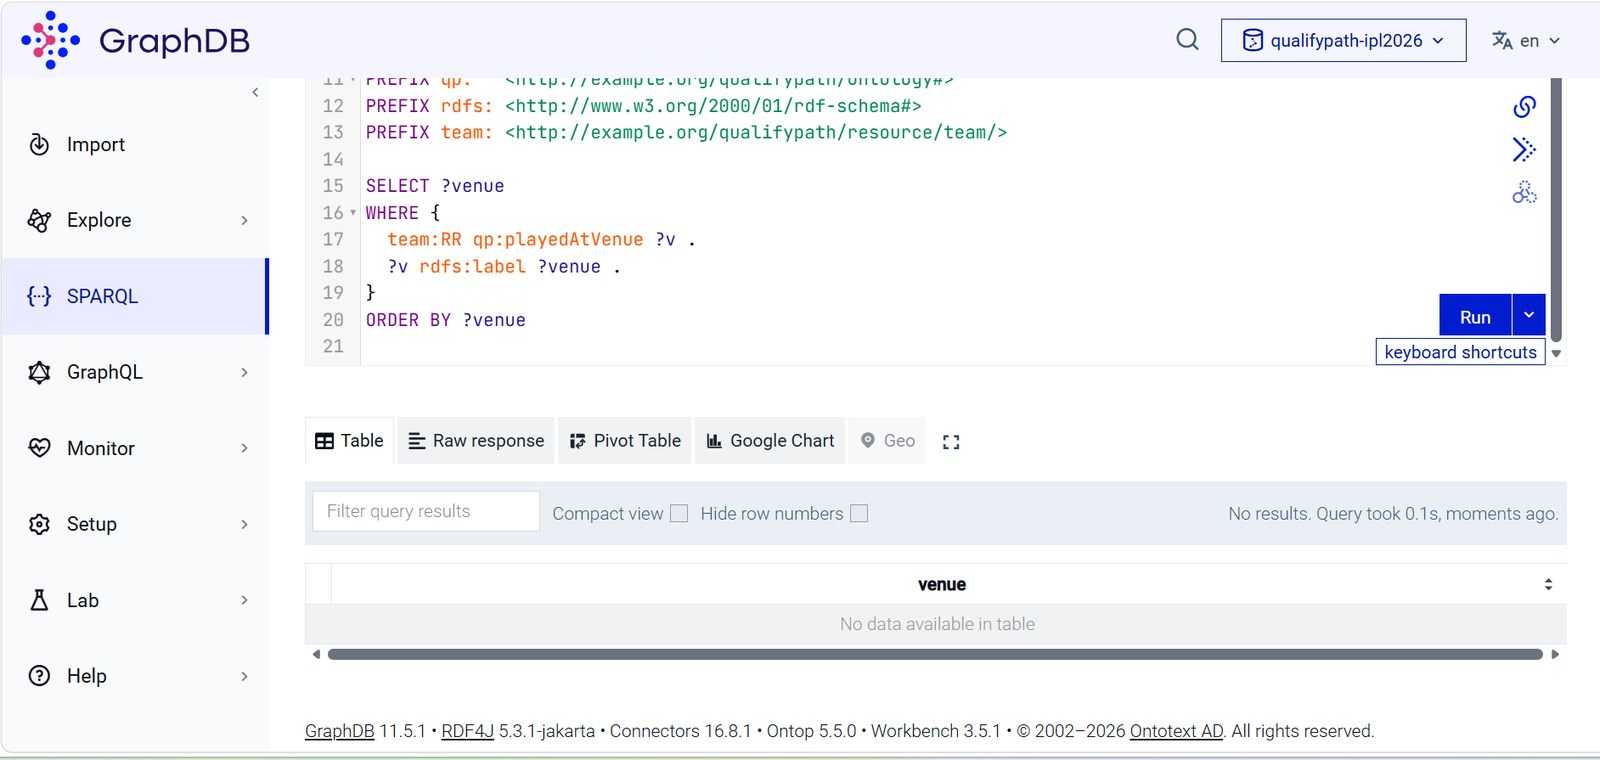
\includegraphics[width=0.49\linewidth]{figures/graphdb_inference_I3_off.jpg}\hfill
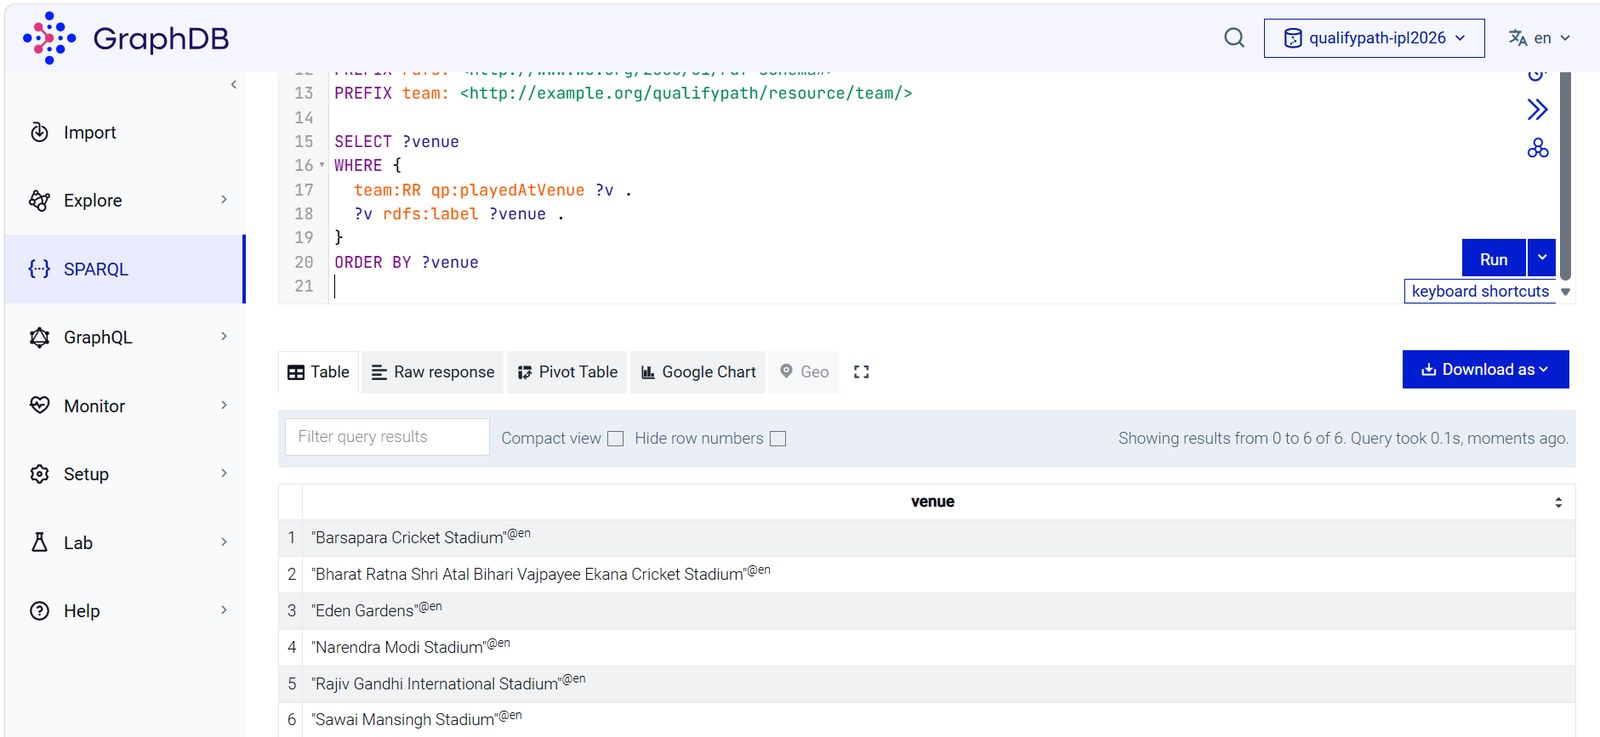
\includegraphics[width=0.49\linewidth]{figures/graphdb_inference_I3_on.jpg}
\caption{I3 in GraphDB with \emph{Include inferred data} off (left, no results) and on (right, six venues).}
\end{figure}
\begin{figure}[H]\centering
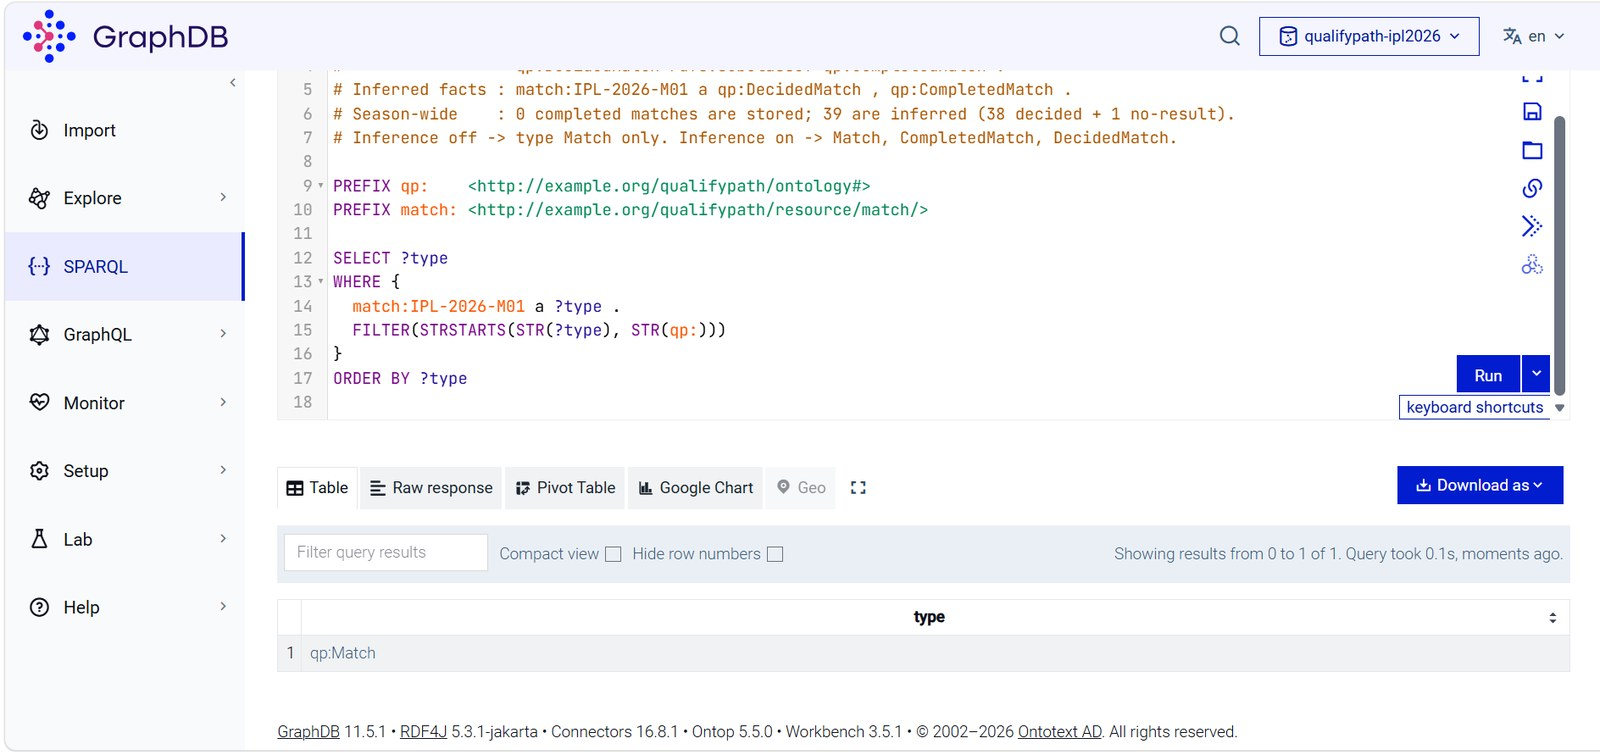
\includegraphics[width=0.49\linewidth]{figures/graphdb_inference_I2_off.jpg}\hfill
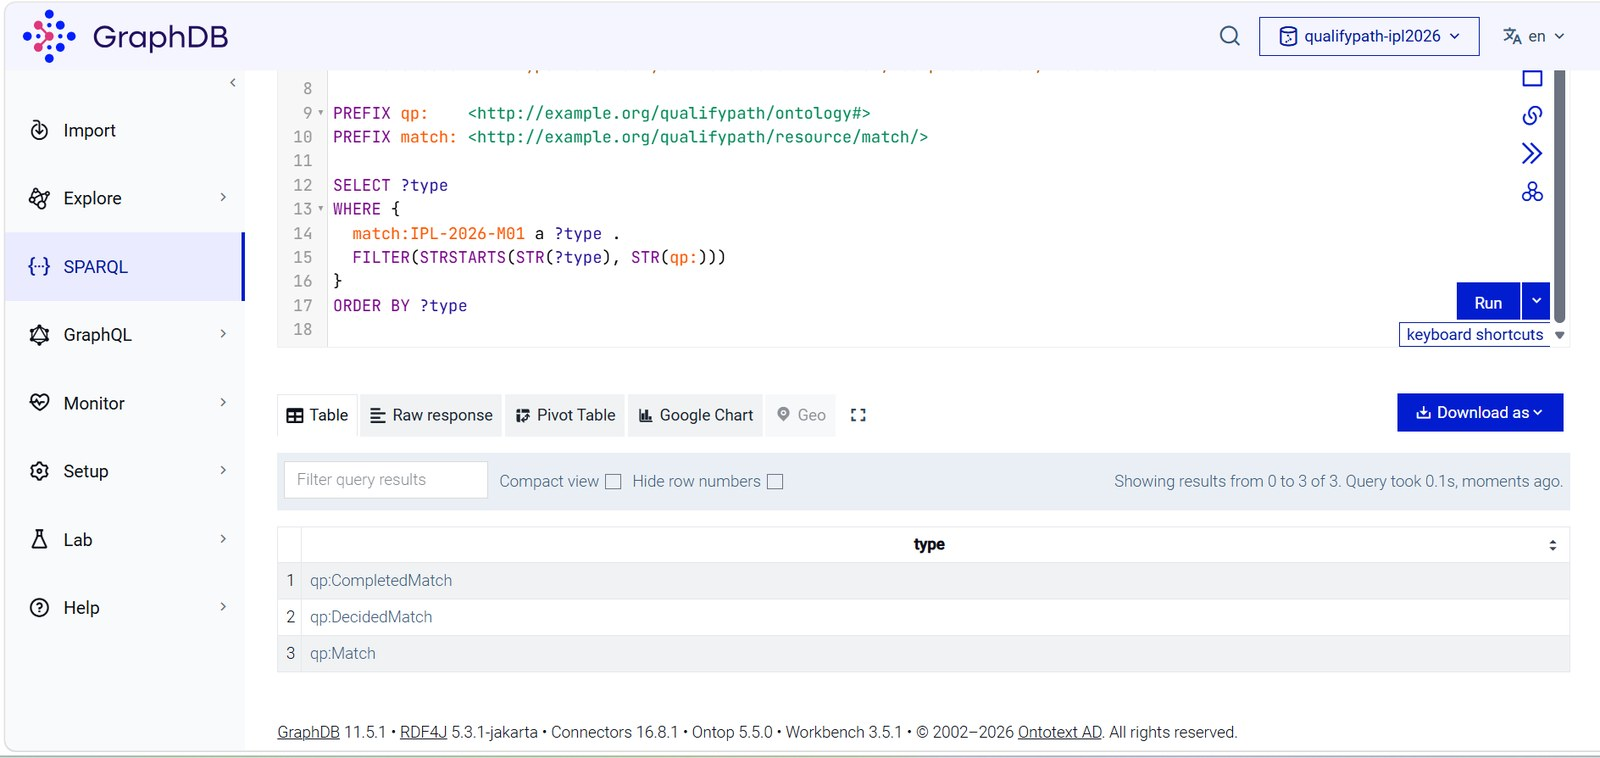
\includegraphics[width=0.49\linewidth]{figures/graphdb_inference_I2_on.jpg}
\caption{I2 in GraphDB: match~1 is only a \texttt{qp:Match} when inference is off, and also a
\texttt{CompletedMatch} and \texttt{DecidedMatch} when it is on.}
\end{figure}
